\documentclass[tikz]{standalone}
\usepackage{tikz}
\usepackage{graphicx}

\usetikzlibrary{calc, angles, quotes}
\usetikzlibrary{intersections} % Necessário para achar pontos de cruzamento

\begin{document}

\begin{tikzpicture}
    \node[scale=4] at (0.2,0) {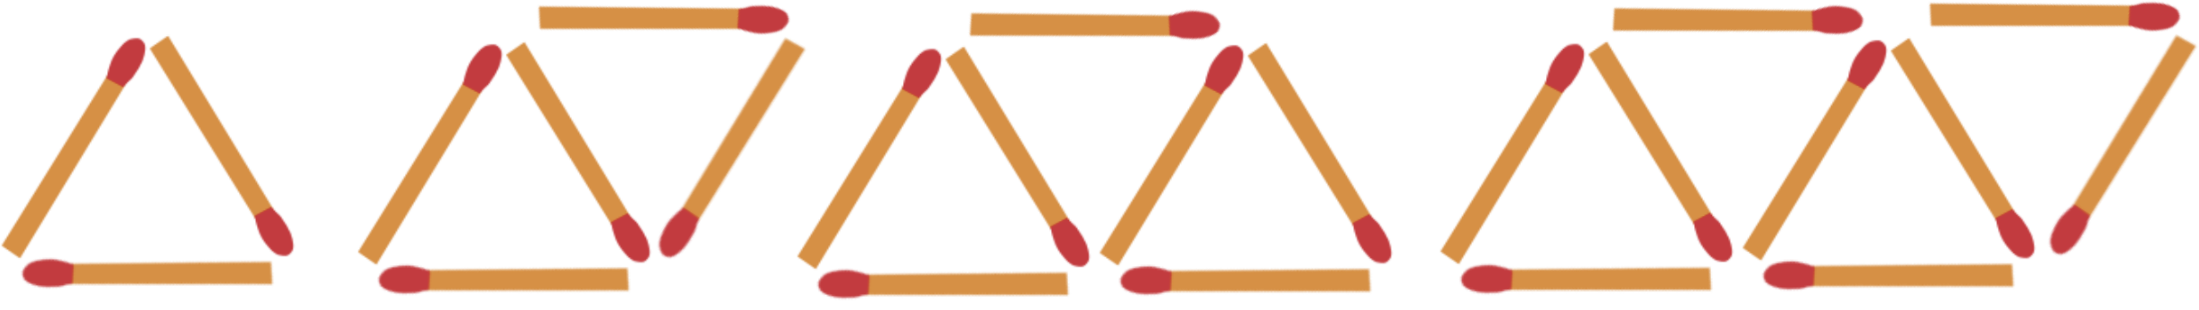
\includegraphics[width=0.25\textwidth]{Simulado_1-atividade_6.png}}; 
    \node at (-5,-1.1) {$(n=1)$};
    \node at (-2.6,-1.1) {$(n=2)$};
    \node at (.2,-1.1) {$(n=3)$};
    \node at (4.2,-1.1) {$(n=4)$};

\end{tikzpicture}
\end{document}